% !TEX root = results_only.tex


describe the results generally

\section{Control case - uniform risk on a uniform population}

\begin{figure}[tb]
    \centering
    \begin{subfigure}[t]{0.45\textwidth}
    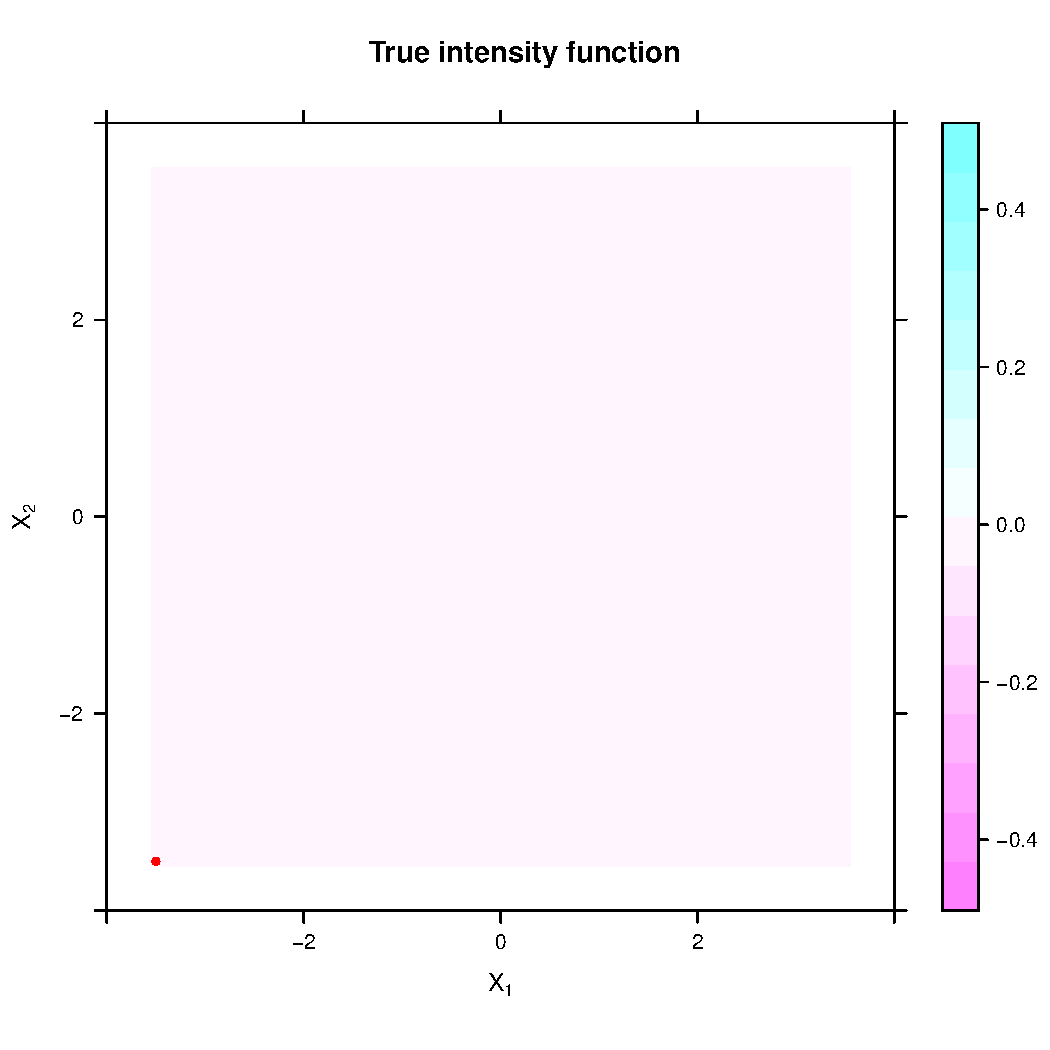
\includegraphics[width=\textwidth]{results/unif_100_1_unif/output/true_intensity_heatmap}
    \caption{True intensity}
    \end{subfigure}
    \begin{subfigure}[t]{0.45\textwidth}
    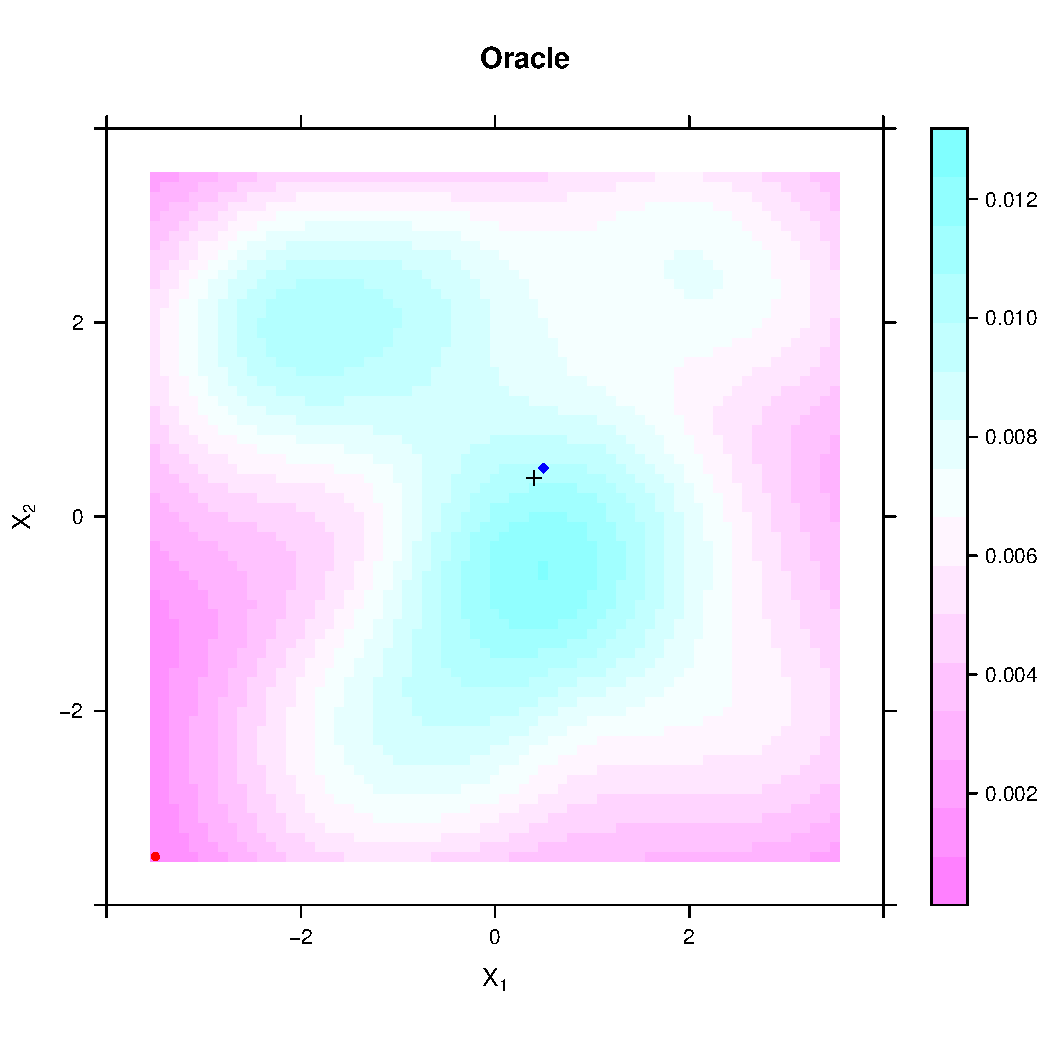
\includegraphics[width=\textwidth]{results/unif_100_1_unif/output/oracle_intensity_heatmap}
    \caption{Oracle estimate}
    \end{subfigure}
    \begin{subfigure}[b]{0.45\textwidth}
    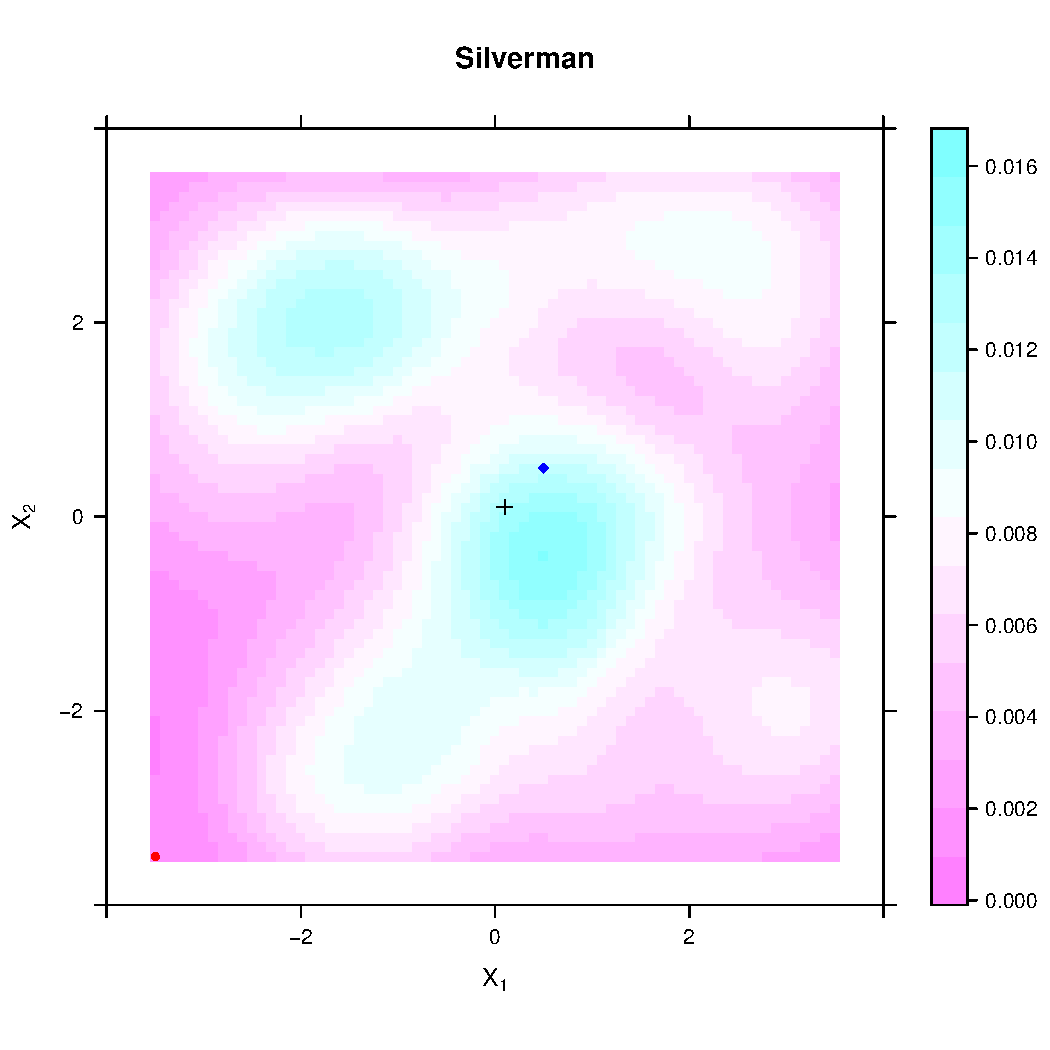
\includegraphics[width=\textwidth]{results/unif_100_1_unif/output/silverman_intensity_heatmap}
    \caption{Silverman estimate}
    \end{subfigure}
    \begin{subfigure}[b]{0.45\textwidth}
    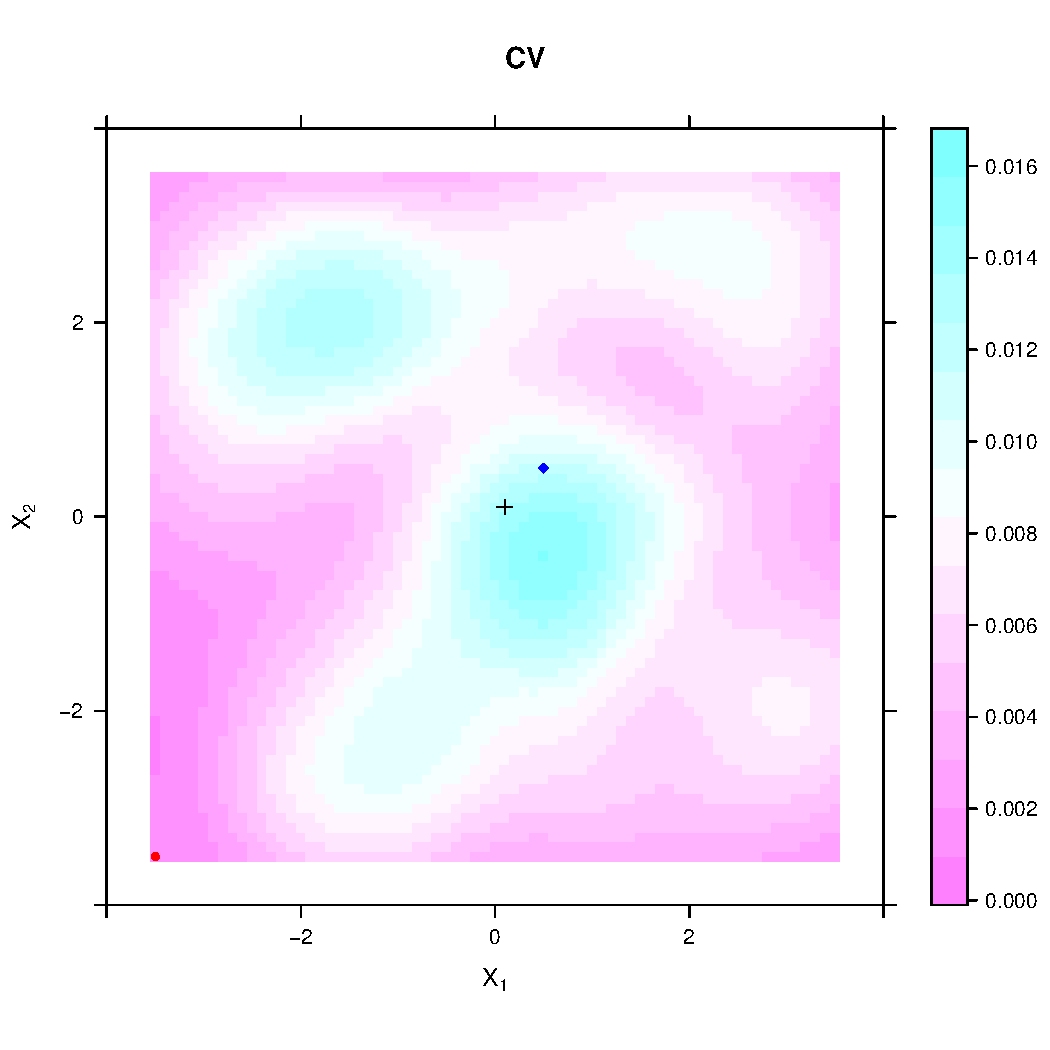
\includegraphics[width=\textwidth]{results/unif_100_1_unif/output/CV_intensity_heatmap}
    \caption{Cross-validation estimate}
    \end{subfigure}
    \label{fig:cases_unif_100_unif}
    \caption{Example cases: uniform intensity on uniform population, 100 cases}
\end{figure}

\begin{figure}[tb]
    \centering
    \begin{subfigure}[b]{0.45\textwidth}
    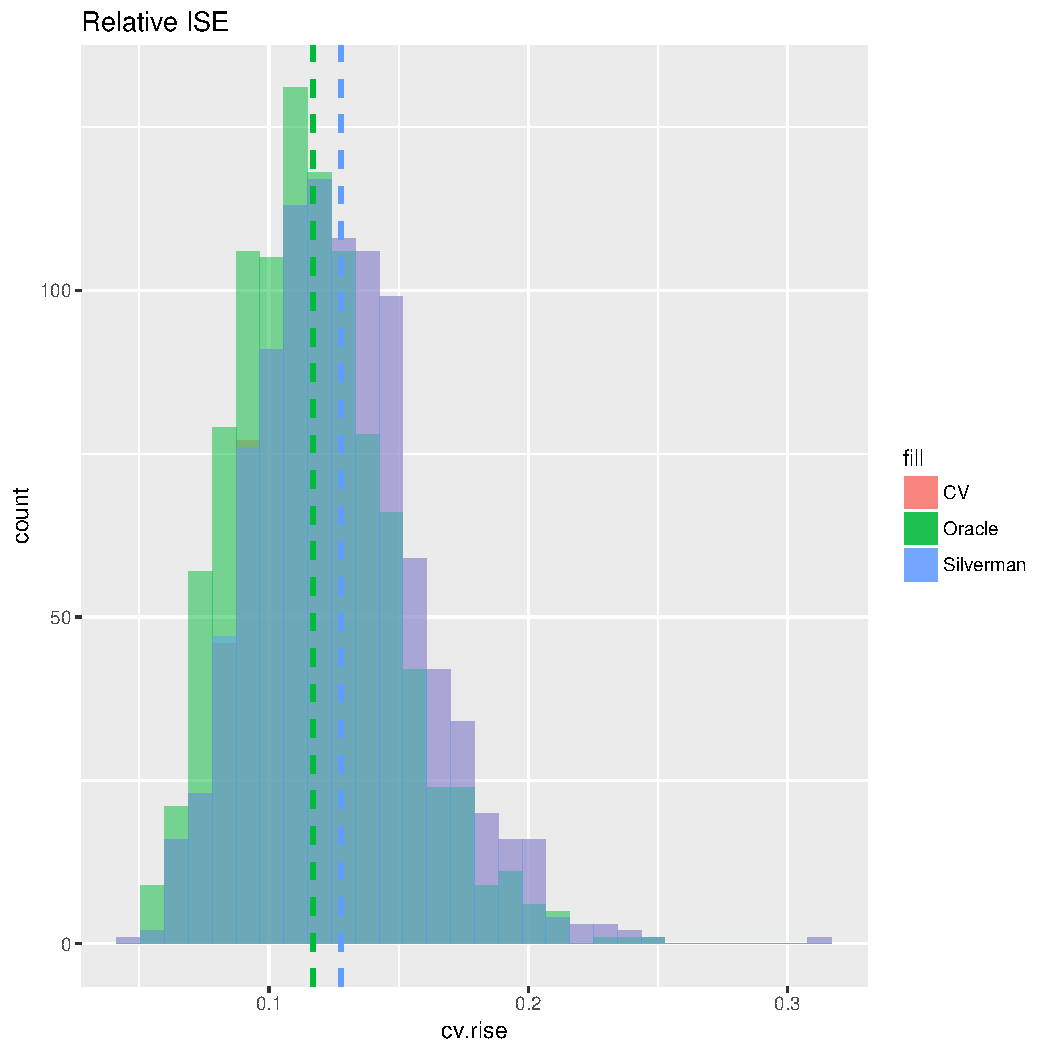
\includegraphics[width=\textwidth]{results/unif_100_1_unif/output/ise-relative-histogram}
    \caption{Relative ISE}
    \end{subfigure}
    \begin{subfigure}[b]{0.45\textwidth}
    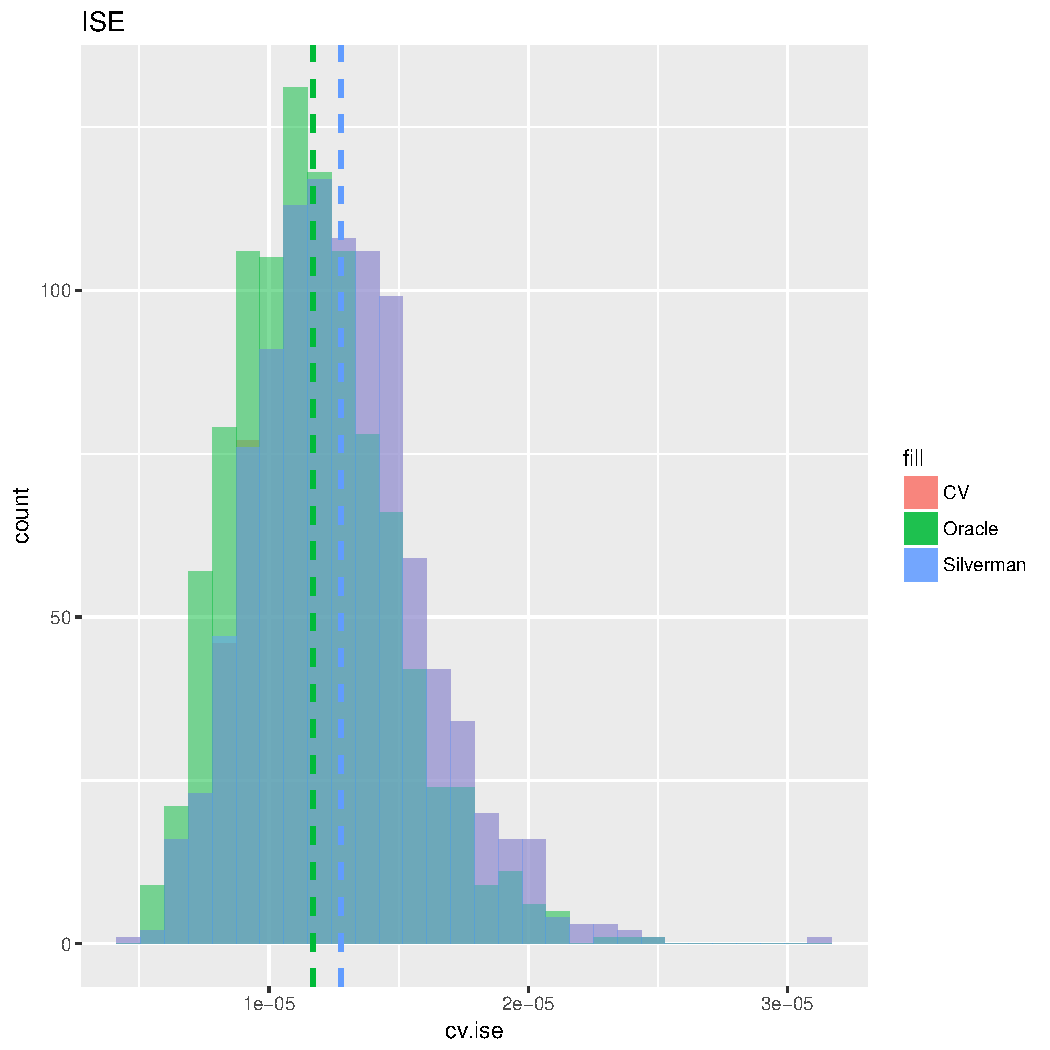
\includegraphics[width=\textwidth]{results/unif_100_1_unif/output/ise-histogram}
    \caption{Absolute ISE}
    \end{subfigure}
    \caption[ISE: uniform on uniform]{Integrated squared error histogram for uniform intensity on a uniform population, 100 cases}
    \label{fig:ise_unif_100_1_unif}
\end{figure}

\section{Single-peak risk on a uniform population}
% latex table generated in R 3.4.0 by xtable 1.8-2 package
% Sat Aug  5 21:15:22 2017
\begin{tabular}{lrrr}
  \hline
 & Oracle & Silverman & CV \\ 
  \hline
MISE & 0.000022 & 0.000035 & 0.000034 \\ 
  Relative MISE & 0.003358 & 0.005293 & 0.005266 \\ 
  MIAE & 0.002505 & 0.003100 & 0.003092 \\ 
  Relative MIAE & 0.031010 & 0.038378 & 0.038279 \\ 
  Max Error & 0.020705 & 0.030617 & 0.030498 \\ 
  Peak bias & -0.012292 & 0.006167 & 0.006026 \\ 
  Relative Peak bias & -0.152166 & 0.076337 & 0.074592 \\ 
  Peak drift & 0.265067 & 0.409888 & 0.408051 \\ 
  Relative Peak drift & 0.037867 & 0.058555 & 0.058293 \\ 
  Centroid bias & -0.012639 & -0.000422 & -0.000492 \\ 
  Relative Centroid bias & -0.156464 & -0.005226 & -0.006090 \\ 
  Centroid drift & 0.199485 & 0.216521 & 0.216495 \\ 
  Relative Centroid drift & 0.028498 & 0.030932 & 0.030928 \\ 
   \hline
\end{tabular}


\section{Varying the number of cases}

\subsection{50 cases}
% latex table generated in R 3.4.0 by xtable 1.8-2 package
% Sat Aug  5 19:49:51 2017
\begin{table}[ht]
\centering
\begin{tabular}{rrrr}
  \hline
 & Oracle & Silverman & CV \\ 
  \hline
MISE & 0.000008 & 0.000014 & 0.000014 \\ 
  Relative MISE & 0.005208 & 0.008600 & 0.008580 \\ 
  MIAE & 0.001568 & 0.001955 & 0.001953 \\ 
  Relative MIAE & 0.038833 & 0.048413 & 0.048363 \\ 
  Max Error & 0.012435 & 0.018787 & 0.018756 \\ 
  Peak bias & -0.007124 & 0.004056 & 0.004020 \\ 
  Relative Peak bias & -0.176378 & 0.100410 & 0.099522 \\ 
  Peak drift & 0.322404 & 0.476198 & 0.475222 \\ 
  Relative Peak drift & 0.046058 & 0.068028 & 0.067889 \\ 
  Centroid bias & -0.007304 & 0.000496 & 0.000487 \\ 
  Relative Centroid bias & -0.180839 & 0.012284 & 0.012057 \\ 
  Centroid drift & 0.262196 & 0.280772 & 0.281105 \\ 
  Relative Centroid drift & 0.037457 & 0.040110 & 0.040158 \\ 
   \hline
\end{tabular}
\caption{Mean error rates} 
\label{tbl:mean_error_rates}
\end{table}


\subsection{100 cases}
% latex table generated in R 3.4.0 by xtable 1.8-2 package
% Sat Aug  5 21:15:22 2017
\begin{tabular}{lrrr}
  \hline
 & Oracle & Silverman & CV \\ 
  \hline
MISE & 0.000022 & 0.000035 & 0.000034 \\ 
  Relative MISE & 0.003358 & 0.005293 & 0.005266 \\ 
  MIAE & 0.002505 & 0.003100 & 0.003092 \\ 
  Relative MIAE & 0.031010 & 0.038378 & 0.038279 \\ 
  Max Error & 0.020705 & 0.030617 & 0.030498 \\ 
  Peak bias & -0.012292 & 0.006167 & 0.006026 \\ 
  Relative Peak bias & -0.152166 & 0.076337 & 0.074592 \\ 
  Peak drift & 0.265067 & 0.409888 & 0.408051 \\ 
  Relative Peak drift & 0.037867 & 0.058555 & 0.058293 \\ 
  Centroid bias & -0.012639 & -0.000422 & -0.000492 \\ 
  Relative Centroid bias & -0.156464 & -0.005226 & -0.006090 \\ 
  Centroid drift & 0.199485 & 0.216521 & 0.216495 \\ 
  Relative Centroid drift & 0.028498 & 0.030932 & 0.030928 \\ 
   \hline
\end{tabular}


\subsection{200 cases}
% latex table generated in R 3.4.0 by xtable 1.8-2 package
% Sat Aug  5 21:44:37 2017
\begin{table}[H]
\centering
\begin{tabular}{lrrr}
  \hline
 & Oracle & Silverman & CV \\ 
  \hline
MISE & 0.000053 & 0.000083 & 0.000082 \\ 
  Relative MISE & 0.002029 & 0.003184 & 0.003129 \\ 
  MIAE & 0.003909 & 0.004852 & 0.004810 \\ 
  Relative MIAE & 0.024196 & 0.030032 & 0.029772 \\ 
  Max Error & 0.033936 & 0.049447 & 0.048810 \\ 
  Peak bias & -0.016473 & 0.010215 & 0.009458 \\ 
  Relative Peak bias & -0.101961 & 0.063224 & 0.058539 \\ 
  Peak drift & 0.219372 & 0.357137 & 0.353058 \\ 
  Relative Peak drift & 0.031339 & 0.051020 & 0.050437 \\ 
  Centroid bias & -0.017532 & -0.001587 & -0.001859 \\ 
  Relative Centroid bias & -0.108518 & -0.009821 & -0.011508 \\ 
  Centroid drift & 0.146327 & 0.158930 & 0.158287 \\ 
  Relative Centroid drift & 0.020904 & 0.022704 & 0.022612 \\ 
   \hline
\end{tabular}
\caption{Mean error rates} 
\label{tbl:mean_error_rates}
\end{table}


\subsection{500 cases}
% latex table generated in R 3.4.0 by xtable 1.8-2 package
% Sat Aug  5 22:43:32 2017
\begin{table}[ht]
\centering
\begin{tabular}{rrrr}
  \hline
 & Oracle & Silverman & CV \\ 
  \hline
MISE & 0.000170 & 0.000265 & 0.000244 \\ 
  Relative MISE & 0.001041 & 0.001626 & 0.001496 \\ 
  MIAE & 0.007096 & 0.008775 & 0.008421 \\ 
  Relative MIAE & 0.017567 & 0.021725 & 0.020849 \\ 
  Max Error & 0.065158 & 0.092681 & 0.087429 \\ 
  Peak bias & -0.023250 & 0.018688 & 0.012450 \\ 
  Relative Peak bias & -0.057562 & 0.046269 & 0.030824 \\ 
  Peak drift & 0.176919 & 0.293212 & 0.276800 \\ 
  Relative Peak drift & 0.025274 & 0.041887 & 0.039543 \\ 
  Centroid bias & -0.026539 & -0.003605 & -0.005705 \\ 
  Relative Centroid bias & -0.065707 & -0.008925 & -0.014124 \\ 
  Centroid drift & 0.096196 & 0.104184 & 0.103456 \\ 
  Relative Centroid drift & 0.013742 & 0.014883 & 0.014779 \\ 
   \hline
\end{tabular}
\caption{Mean error rates} 
\label{tbl:mean_error_rates}
\end{table}


\subsection{1000 cases}
% latex table generated in R 3.4.0 by xtable 1.8-2 package
% Sun Aug  6 00:15:05 2017
\begin{table}[ht]
\centering
\begin{tabular}{lrrr}
  \hline
 & Oracle & Silverman & CV \\ 
  \hline
MISE & 0.000379 & 0.000619 & 0.000484 \\ 
  Relative MISE & 0.000581 & 0.000948 & 0.000742 \\ 
  MIAE & 0.010804 & 0.013570 & 0.012061 \\ 
  Relative MIAE & 0.013375 & 0.016798 & 0.014931 \\ 
  Max Error & 0.105433 & 0.145677 & 0.126060 \\ 
  Peak bias & -0.034129 & 0.024518 & -0.000092 \\ 
  Relative Peak bias & -0.042248 & 0.030351 & -0.000114 \\ 
  Peak drift & 0.129044 & 0.251876 & 0.185739 \\ 
  Relative Peak drift & 0.018435 & 0.035982 & 0.026534 \\ 
  Centroid bias & -0.037516 & -0.001969 & -0.014152 \\ 
  Relative Centroid bias & -0.046441 & -0.002438 & -0.017519 \\ 
  Centroid drift & 0.068889 & 0.076451 & 0.074548 \\ 
  Relative Centroid drift & 0.009841 & 0.010922 & 0.010650 \\ 
   \hline
\end{tabular}
\caption{Mean error rates} 
\label{tbl:mean_error_rates}
\end{table}


\section{Varying the size of the population}

\subsection{100 cases from 10,000}
% latex table generated in R 3.4.0 by xtable 1.8-2 package
% Sat Aug  5 21:15:22 2017
\begin{tabular}{lrrr}
  \hline
 & Oracle & Silverman & CV \\ 
  \hline
MISE & 0.000022 & 0.000035 & 0.000034 \\ 
  Relative MISE & 0.003358 & 0.005293 & 0.005266 \\ 
  MIAE & 0.002505 & 0.003100 & 0.003092 \\ 
  Relative MIAE & 0.031010 & 0.038378 & 0.038279 \\ 
  Max Error & 0.020705 & 0.030617 & 0.030498 \\ 
  Peak bias & -0.012292 & 0.006167 & 0.006026 \\ 
  Relative Peak bias & -0.152166 & 0.076337 & 0.074592 \\ 
  Peak drift & 0.265067 & 0.409888 & 0.408051 \\ 
  Relative Peak drift & 0.037867 & 0.058555 & 0.058293 \\ 
  Centroid bias & -0.012639 & -0.000422 & -0.000492 \\ 
  Relative Centroid bias & -0.156464 & -0.005226 & -0.006090 \\ 
  Centroid drift & 0.199485 & 0.216521 & 0.216495 \\ 
  Relative Centroid drift & 0.028498 & 0.030932 & 0.030928 \\ 
   \hline
\end{tabular}


\subsection{1000 cases from 100,000}
% latex table generated in R 3.4.0 by xtable 1.8-2 package
% Sun Aug  6 00:13:35 2017
\begin{table}[ht]
\centering
\begin{tabular}{lrrr}
  \hline
 & Oracle & Silverman & CV \\ 
  \hline
MISE & 0.000005 & 0.000007 & 0.000006 \\ 
  Relative MISE & 0.000780 & 0.001138 & 0.000957 \\ 
  MIAE & 0.001194 & 0.001443 & 0.001318 \\ 
  Relative MIAE & 0.014783 & 0.017860 & 0.016319 \\ 
  Max Error & 0.012033 & 0.016294 & 0.014388 \\ 
  Peak bias & -0.006071 & 0.001338 & -0.001420 \\ 
  Relative Peak bias & -0.075150 & 0.016561 & -0.017584 \\ 
  Peak drift & 0.191971 & 0.283546 & 0.257819 \\ 
  Relative Peak drift & 0.027424 & 0.040507 & 0.036831 \\ 
  Centroid bias & -0.007017 & -0.003590 & -0.004719 \\ 
  Relative Centroid bias & -0.086858 & -0.044443 & -0.058412 \\ 
  Centroid drift & 0.077427 & 0.087651 & 0.084033 \\ 
  Relative Centroid drift & 0.011061 & 0.012522 & 0.012005 \\ 
   \hline
\end{tabular}
\caption{Mean error rates} 
\label{tbl:mean_error_rates}
\end{table}


\section{Varying the decay of the risk function}

\subsection{100 cases with decay rate 0.5}
% latex table generated in R 3.4.0 by xtable 1.8-2 package
% Sun Jul 30 10:54:52 2017
\begin{table}[ht]
\centering
\begin{tabular}{rrrr}
  \hline
 & Oracle & Silverman & CV \\ 
  \hline
MISE & 0.000036 & 0.000046 & 0.000063 \\ 
  Relative MISE & 0.000340 & 0.000438 & 0.000607 \\ 
  MIAE & 0.000466 & 0.000425 & 0.000563 \\ 
  Relative MIAE & 0.001442 & 0.001314 & 0.001741 \\ 
  Max Error & 0.023200 & 0.030300 & 0.039341 \\ 
  Peak bias & 0.032038 & 0.050895 & 0.055081 \\ 
  Relative Peak bias & 0.099132 & 0.157480 & 0.170430 \\ 
  Peak drift & 0.080767 & 0.118526 & 0.114042 \\ 
  Relative Peak drift & 0.011538 & 0.016932 & 0.016292 \\ 
  Centroid bias & 0.033350 & 0.057284 & 0.053665 \\ 
  Relative Centroid bias & 0.103192 & 0.177250 & 0.166049 \\ 
  Centroid drift & 0.056974 & 0.058126 & 0.057936 \\ 
  Relative Centroid drift & 0.008139 & 0.008304 & 0.008277 \\ 
   \hline
\end{tabular}
\caption{Standard deviation of error rates} 
\label{tbl:stddev_error_rates}
\end{table}


\subsection{100 cases with decay rate 0.7}
% latex table generated in R 3.4.0 by xtable 1.8-2 package
% Sat Aug  5 20:24:52 2017
\begin{table}[ht]
\centering
\begin{tabular}{lrrr}
  \hline
 & Oracle & Silverman & CV \\ 
  \hline
MISE & 0.000041 & 0.000070 & 0.000068 \\ 
  Relative MISE & 0.001509 & 0.002587 & 0.002508 \\ 
  MIAE & 0.002424 & 0.003082 & 0.003036 \\ 
  Relative MIAE & 0.014708 & 0.018700 & 0.018421 \\ 
  Max Error & 0.040419 & 0.063188 & 0.061764 \\ 
  Peak bias & -0.024625 & 0.014782 & 0.013157 \\ 
  Relative Peak bias & -0.149402 & 0.089681 & 0.079821 \\ 
  Peak drift & 0.178185 & 0.309841 & 0.306002 \\ 
  Relative Peak drift & 0.025455 & 0.044263 & 0.043715 \\ 
  Centroid bias & -0.026327 & -0.008016 & -0.008467 \\ 
  Relative Centroid bias & -0.159727 & -0.048632 & -0.051370 \\ 
  Centroid drift & 0.110594 & 0.115124 & 0.114988 \\ 
  Relative Centroid drift & 0.015799 & 0.016446 & 0.016427 \\ 
   \hline
\end{tabular}
\caption{Mean error rates} 
\label{tbl:mean_error_rates}
\end{table}


\subsection{100 cases with decay rate 1.0}
% latex table generated in R 3.4.0 by xtable 1.8-2 package
% Sat Aug  5 21:15:22 2017
\begin{tabular}{lrrr}
  \hline
 & Oracle & Silverman & CV \\ 
  \hline
MISE & 0.000022 & 0.000035 & 0.000034 \\ 
  Relative MISE & 0.003358 & 0.005293 & 0.005266 \\ 
  MIAE & 0.002505 & 0.003100 & 0.003092 \\ 
  Relative MIAE & 0.031010 & 0.038378 & 0.038279 \\ 
  Max Error & 0.020705 & 0.030617 & 0.030498 \\ 
  Peak bias & -0.012292 & 0.006167 & 0.006026 \\ 
  Relative Peak bias & -0.152166 & 0.076337 & 0.074592 \\ 
  Peak drift & 0.265067 & 0.409888 & 0.408051 \\ 
  Relative Peak drift & 0.037867 & 0.058555 & 0.058293 \\ 
  Centroid bias & -0.012639 & -0.000422 & -0.000492 \\ 
  Relative Centroid bias & -0.156464 & -0.005226 & -0.006090 \\ 
  Centroid drift & 0.199485 & 0.216521 & 0.216495 \\ 
  Relative Centroid drift & 0.028498 & 0.030932 & 0.030928 \\ 
   \hline
\end{tabular}


\subsection{100 cases with decay rate 1.4}
% latex table generated in R 3.4.3 by xtable 1.8-2 package
% Sun Apr 15 09:02:16 2018
\begin{tabular}{lrrr}
  \toprule
 & Oracle & Silverman & CV \\ 
  \midrule
MISE & 0.000012 & 0.000019 & 0.000016 \\ 
  Relative MISE & 0.006627 & 0.010652 & 0.009328 \\ 
  Normalized MISE & 1.162791 & 1.869138 & 1.636752 \\ 
  MIAE & 0.002291 & 0.002949 & 0.002662 \\ 
  Relative MIAE & 0.054683 & 0.070397 & 0.063559 \\ 
  Normalized MIAE & 0.000023 & 0.000029 & 0.000027 \\ 
  Supremum error & 0.011293 & 0.016460 & 0.014595 \\ 
  Normalized Sup error & 0.000113 & 0.000165 & 0.000146 \\ 
  Peak bias & -0.005739 & 0.003331 & -0.001423 \\ 
  Relative Peak bias & -0.137007 & 0.079526 & -0.033973 \\ 
  Peak drift & 0.407527 & 0.576641 & 0.466724 \\ 
  Relative Peak drift & 0.058218 & 0.082377 & 0.066675 \\ 
  Centroid bias & -0.005876 & 0.001197 & -0.003106 \\ 
  Relative Centroid bias & -0.140265 & 0.028578 & -0.074149 \\ 
  Centroid drift & 0.337723 & 0.384568 & 0.351105 \\ 
  Relative Centroid drift & 0.048246 & 0.054938 & 0.050158 \\ 
   \bottomrule
\end{tabular}


\subsection{100 cases with decay rate 2.0}
% latex table generated in R 3.4.0 by xtable 1.8-2 package
% Sat Aug  5 21:31:40 2017
\begin{table}[H]
\centering
\begin{tabular}{lrrr}
  \hline
 & Oracle & Silverman & CV \\ 
  \hline
MISE & 0.000006 & 0.000012 & 0.000012 \\ 
  Relative MISE & 0.011308 & 0.021333 & 0.021316 \\ 
  MIAE & 0.001867 & 0.002638 & 0.002637 \\ 
  Relative MIAE & 0.079514 & 0.112328 & 0.112282 \\ 
  Max Error & 0.006153 & 0.010407 & 0.010401 \\ 
  Peak bias & -0.003225 & 0.003258 & 0.003251 \\ 
  Relative Peak bias & -0.137322 & 0.138713 & 0.138426 \\ 
  Peak drift & 0.615800 & 0.900437 & 0.900381 \\ 
  Relative Peak drift & 0.087971 & 0.128634 & 0.128626 \\ 
  Centroid bias & -0.003271 & 0.001927 & 0.001923 \\ 
  Relative Centroid bias & -0.139292 & 0.082052 & 0.081892 \\ 
  Centroid drift & 0.534199 & 0.668770 & 0.668461 \\ 
  Relative Centroid drift & 0.076314 & 0.095539 & 0.095494 \\ 
   \hline
\end{tabular}
\caption{Mean error rates} 
\label{tbl:mean_error_rates}
\end{table}


\section{Varying the decay of the population density}

\subsection{100 cases with uniform population}
% latex table generated in R 3.4.0 by xtable 1.8-2 package
% Sat Aug  5 21:15:22 2017
\begin{tabular}{lrrr}
  \hline
 & Oracle & Silverman & CV \\ 
  \hline
MISE & 0.000022 & 0.000035 & 0.000034 \\ 
  Relative MISE & 0.003358 & 0.005293 & 0.005266 \\ 
  MIAE & 0.002505 & 0.003100 & 0.003092 \\ 
  Relative MIAE & 0.031010 & 0.038378 & 0.038279 \\ 
  Max Error & 0.020705 & 0.030617 & 0.030498 \\ 
  Peak bias & -0.012292 & 0.006167 & 0.006026 \\ 
  Relative Peak bias & -0.152166 & 0.076337 & 0.074592 \\ 
  Peak drift & 0.265067 & 0.409888 & 0.408051 \\ 
  Relative Peak drift & 0.037867 & 0.058555 & 0.058293 \\ 
  Centroid bias & -0.012639 & -0.000422 & -0.000492 \\ 
  Relative Centroid bias & -0.156464 & -0.005226 & -0.006090 \\ 
  Centroid drift & 0.199485 & 0.216521 & 0.216495 \\ 
  Relative Centroid drift & 0.028498 & 0.030932 & 0.030928 \\ 
   \hline
\end{tabular}


\subsection{100 cases with population decay rate 2.0}
% latex table generated in R 3.4.0 by xtable 1.8-2 package
% Sat Aug  5 21:07:06 2017
\begin{tabular}{lrrr}
  \hline
 & Oracle & Silverman & CV \\ 
  \hline
MISE & 0.000021 & 0.000034 & 0.000034 \\ 
  Relative MISE & 0.003273 & 0.005274 & 0.005179 \\ 
  MIAE & 0.002642 & 0.003221 & 0.003194 \\ 
  Relative MIAE & 0.032700 & 0.039874 & 0.039542 \\ 
  Max Error & 0.020044 & 0.030183 & 0.029789 \\ 
  Peak bias & -0.009647 & 0.006342 & 0.005880 \\ 
  Relative Peak bias & -0.119422 & 0.078502 & 0.072792 \\ 
  Peak drift & 0.309850 & 0.468400 & 0.464955 \\ 
  Relative Peak drift & 0.044264 & 0.066914 & 0.066422 \\ 
  Centroid bias & -0.010650 & -0.004896 & -0.004979 \\ 
  Relative Centroid bias & -0.131838 & -0.060607 & -0.061636 \\ 
  Centroid drift & 0.192663 & 0.192580 & 0.192641 \\ 
  Relative Centroid drift & 0.027523 & 0.027511 & 0.027520 \\ 
   \hline
\end{tabular}


\subsection{100 cases with population decay rate 1.4}
% latex table generated in R 3.4.0 by xtable 1.8-2 package
% Sat Aug  5 21:37:13 2017
\begin{table}[ht]
\centering
\begin{tabular}{lrrr}
  \hline
 & Oracle & Silverman & CV \\ 
  \hline
MISE & 0.000023 & 0.000036 & 0.000034 \\ 
  Relative MISE & 0.003558 & 0.005476 & 0.005188 \\ 
  MIAE & 0.002836 & 0.003304 & 0.003227 \\ 
  Relative MIAE & 0.035109 & 0.040906 & 0.039946 \\ 
  Max Error & 0.019837 & 0.031477 & 0.030030 \\ 
  Peak bias & -0.008783 & 0.006794 & 0.005493 \\ 
  Relative Peak bias & -0.108731 & 0.084104 & 0.067997 \\ 
  Peak drift & 0.279824 & 0.422472 & 0.412451 \\ 
  Relative Peak drift & 0.039975 & 0.060353 & 0.058922 \\ 
  Centroid bias & -0.009989 & -0.004347 & -0.004578 \\ 
  Relative Centroid bias & -0.123654 & -0.053816 & -0.056672 \\ 
  Centroid drift & 0.154247 & 0.149632 & 0.149878 \\ 
  Relative Centroid drift & 0.022035 & 0.021376 & 0.021411 \\ 
   \hline
\end{tabular}
\caption{Mean error rates} 
\label{tbl:mean_error_rates}
\end{table}


\subsection{100 cases with population decay rate 1.0}
% latex table generated in R 3.4.0 by xtable 1.8-2 package
% Sun Jul 30 15:44:25 2017
\begin{table}[ht]
\centering
\begin{tabular}{rrrr}
  \hline
 & Oracle & Silverman & CV \\ 
  \hline
MISE & 0.000057 & 0.000070 & 0.000066 \\ 
  Relative MISE & 0.008716 & 0.010683 & 0.010096 \\ 
  MIAE & 0.000835 & 0.000624 & 0.000695 \\ 
  Relative MIAE & 0.010332 & 0.007724 & 0.008599 \\ 
  Max Error & 0.039895 & 0.059402 & 0.054207 \\ 
  Peak bias & 0.028142 & 0.048165 & 0.042352 \\ 
  Relative Peak bias & 0.348370 & 0.596241 & 0.524281 \\ 
  Peak drift & 1.182271 & 1.214951 & 1.199142 \\ 
  Relative Peak drift & 0.168896 & 0.173564 & 0.171306 \\ 
  Centroid bias & 0.007869 & 0.010140 & 0.009436 \\ 
  Relative Centroid bias & 0.097406 & 0.125528 & 0.116811 \\ 
  Centroid drift & 0.218588 & 0.158346 & 0.171699 \\ 
  Relative Centroid drift & 0.031227 & 0.022621 & 0.024528 \\ 
   \hline
\end{tabular}
\caption{Standard deviation of error rates} 
\label{tbl:stddev_error_rates}
\end{table}


\subsection{100 cases with population decay rate 0.7}
% latex table generated in R 3.4.0 by xtable 1.8-2 package
% Sat Aug  5 23:40:16 2017
\begin{table}[H]
\centering
\begin{tabular}{lrrr}
  \hline
 & Oracle & Silverman & CV \\ 
  \hline
MISE & 0.001551 & 0.001488 & 13455866197.588720 \\ 
  Relative MISE & 0.237723 & 0.227961 & 2062001845964.798828 \\ 
  MIAE & 0.006198 & 0.006264 & 516.211152 \\ 
  Relative MIAE & 0.076728 & 0.077543 & 6390.223929 \\ 
  Max Error & 0.401935 & 0.425882 & 148124.498061 \\ 
  Peak bias & 0.328253 & 0.352447 & 0.302431 \\ 
  Relative Peak bias & 4.063469 & 4.362974 & 3.743822 \\ 
  Peak drift & 2.208545 & 2.202533 & 2.260982 \\ 
  Relative Peak drift & 0.315506 & 0.314648 & 0.322997 \\ 
  Centroid bias & -0.008139 & -0.006532 & -0.013600 \\ 
  Relative Centroid bias & -0.100757 & -0.080862 & -0.168350 \\ 
  Centroid drift & 0.325652 & 0.299875 & 0.438476 \\ 
  Relative Centroid drift & 0.046522 & 0.042839 & 0.062639 \\ 
   \hline
\end{tabular}
\caption{Mean error rates} 
\label{tbl:mean_error_rates}
\end{table}


\section{Varying the distance between two peaks}

\subsection{100 cases in 2 peaks separated by 1}
% latex table generated in R 3.4.2 by xtable 1.8-2 package
% Sat Feb 17 16:39:11 2018
\begin{tabular}{lrrr}
  \hline
 & Oracle & Silverman & CV \\ 
  \hline
MISE & 0.000020 & 0.000028 & 0.000028 \\ 
  Relative MISE & 0.003806 & 0.005434 & 0.005499 \\ 
  Normalized MISE & 0.000020 & 0.000028 & 0.000028 \\ 
  MIAE & 0.002482 & 0.002946 & 0.002911 \\ 
  Relative MIAE & 0.034598 & 0.041069 & 0.040574 \\ 
  Max Error & 0.018613 & 0.025324 & 0.024450 \\ 
  Peak bias & -0.008775 & 0.002958 & -0.002987 \\ 
  Relative Peak bias & -0.122312 & 0.041234 & -0.041636 \\ 
  Peak drift & 0.308419 & 0.424717 & 0.350763 \\ 
  Relative Peak drift & 0.044060 & 0.060674 & 0.050109 \\ 
  Centroid bias & -0.009281 & -0.001295 & -0.007951 \\ 
  Relative Centroid bias & -0.129358 & -0.018055 & -0.110820 \\ 
  Centroid drift & 0.225096 & 0.241028 & 0.222905 \\ 
  Relative Centroid drift & 0.032157 & 0.034433 & 0.031844 \\ 
   \hline
\end{tabular}


\subsection{100 cases in 2 peaks separated by 2}
% latex table generated in R 3.3.3 by xtable 1.8-2 package
% Tue Apr 17 10:55:12 2018
\begin{tabular}{lrrr}
  \toprule
 & Oracle & Silverman & CV \\ 
  \midrule
MISE & 0.000016 & 0.000020 & 0.000022 \\ 
  Relative MISE & 0.005511 & 0.006846 & 0.007379 \\ 
  Normalized MISE & 1.616635 & 2.007979 & 2.164501 \\ 
  MIAE & 0.002448 & 0.002717 & 0.002794 \\ 
  Relative MIAE & 0.045194 & 0.050158 & 0.051596 \\ 
  Normalized MIAE & 0.000024 & 0.000027 & 0.000028 \\ 
  Supremum error & 0.015121 & 0.018267 & 0.018826 \\ 
  Normalized Sup error & 0.000151 & 0.000183 & 0.000188 \\ 
  Peak bias & -0.007114 & -0.000308 & -0.002112 \\ 
  Relative Peak bias & -0.131350 & -0.005688 & -0.038995 \\ 
  Peak drift & 0.435316 & 0.501214 & 0.475627 \\ 
  Relative Peak drift & 0.062188 & 0.071602 & 0.067947 \\ 
  Centroid bias & -0.007333 & -0.001889 & -0.004326 \\ 
  Relative Centroid bias & -0.135394 & -0.034870 & -0.079868 \\ 
  Centroid drift & 0.411449 & 0.405429 & 0.408394 \\ 
  Relative Centroid drift & 0.058778 & 0.057918 & 0.058342 \\ 
   \bottomrule
\end{tabular}


\subsection{100 cases in 2 peaks separated by 3}
% latex table generated in R 3.4.0 by xtable 1.8-2 package
% Sat Aug  5 21:31:15 2017
\begin{table}[ht]
\centering
\begin{tabular}{lrrr}
  \hline
 & Oracle & Silverman & CV \\ 
  \hline
MISE & 0.000018 & 0.000019 & 0.000019 \\ 
  Relative MISE & 0.007368 & 0.007591 & 0.007591 \\ 
  MIAE & 0.002675 & 0.002735 & 0.002735 \\ 
  Relative MIAE & 0.053776 & 0.054989 & 0.054991 \\ 
  Max Error & 0.016647 & 0.016798 & 0.016799 \\ 
  Peak bias & -0.010884 & -0.010384 & -0.010381 \\ 
  Relative Peak bias & -0.218843 & -0.208792 & -0.208735 \\ 
  Peak drift & 0.550466 & 0.541528 & 0.541476 \\ 
  Relative Peak drift & 0.078638 & 0.077361 & 0.077354 \\ 
  Centroid bias & -0.011999 & -0.011748 & -0.011746 \\ 
  Relative Centroid bias & -0.241255 & -0.236209 & -0.236168 \\ 
  Centroid drift & 0.581652 & 0.562239 & 0.562221 \\ 
  Relative Centroid drift & 0.083093 & 0.080320 & 0.080317 \\ 
   \hline
\end{tabular}
\caption{Mean error rates} 
\label{tbl:mean_error_rates}
\end{table}


\subsection{100 cases in 2 peaks separated by 4}
% latex table generated in R 3.4.0 by xtable 1.8-2 package
% Sat Aug  5 21:31:21 2017
\begin{tabular}{lrrr}
  \hline
 & Oracle & Silverman & CV \\ 
  \hline
MISE & 0.000020 & 0.000024 & 0.000024 \\ 
  Relative MISE & 0.007580 & 0.009231 & 0.009226 \\ 
  MIAE & 0.002817 & 0.003101 & 0.003100 \\ 
  Relative MIAE & 0.054725 & 0.060231 & 0.060211 \\ 
  Max Error & 0.017437 & 0.019484 & 0.019477 \\ 
  Peak bias & -0.011002 & -0.017317 & -0.017303 \\ 
  Relative Peak bias & -0.213721 & -0.336389 & -0.336120 \\ 
  Peak drift & 0.709475 & 0.472244 & 0.472127 \\ 
  Relative Peak drift & 0.101354 & 0.067463 & 0.067447 \\ 
  Centroid bias & -0.016026 & -0.019387 & -0.019377 \\ 
  Relative Centroid bias & -0.311302 & -0.376586 & -0.376399 \\ 
  Centroid drift & 0.642990 & 0.505662 & 0.505713 \\ 
  Relative Centroid drift & 0.091856 & 0.072237 & 0.072245 \\ 
   \hline
\end{tabular}



